\chapter{Project Specification}

\section{Overview}
\label{overview}

As mentioned in the introduction, this project aims at implementing a \textbf{Steer-by-Wire automotive system}. In order to achieve this goal, the complete system will be divided into two main parts, which will be mechanically decoupled from each other:

\begin{itemize}
	\item \textit{Human-Interaction Subsystem}: This is the part of the system that takes care of the interaction between the driver and the steering system. In practice, this section will acquire information about the desired steering angle requested by the driver through the steering wheel, and will generate the corresponding steering request to be sent to the Road-Side Subsystem. In addition, this section of the system will take care of exchanging other information with the driver through buttons and displays, allowing a more precise and personalized interaction with the underlying system.
	
	\item \textit{Road-Side Subsystem}: This is the part of the system that takes care of applying the required steering angle to the road wheels. In practice, this section will include the power components needed to physically move the steering mechanism, together with the electronic system required to control this motion. Hardware and software control strategies, together with sensor feedback, will be used to accurately reach the requested steering position while maintaining a smooth and coherent steering behaviour.
\end{itemize}

Following a common automotive approach, the two systems will be electrically interconnected through a CAN bus, providing a robust communication channel between the two physically separated embedded nodes.

The resulting architecture can therefore be considered as a distributed embedded system, in which the two nodes perform different and well-defined local functions. The Human-Interaction Subsystem is responsible for interpreting the driver's steering request, while the Road-Side Subsystem autonomously manages the physical actuation required to reach the requested steering position.

Although the proposed system represents a simplified demonstrator, particular attention will also be given to monitoring and diagnostic capabilities. Redundant sensing, plausibility checks and communication monitoring will be introduced where appropriate, with the objective of reproducing some of the design principles typically required by safety-oriented automotive embedded systems.


\section{Human-Interaction Subsystem}

As introduced in Section~\ref{overview}, the Human-Interaction Subsystem is responsible for the interaction between the driver and the Steer-by-Wire system. Its main input is the steering wheel position requested by the driver, together with additional user inputs used to configure and interact with the system. The subsystem also provides feedback to the driver through the display.

In addition to the human-machine interaction, this subsystem is responsible for generating the steering request and exchanging information with the other nodes of the system. In the simplified architecture considered in this project, the main communication takes place with the Road-Side Subsystem through the CAN bus.

The proposed architecture of the Human-Interaction Subsystem is shown in Figure~\ref{fig:human_side_block_diagram}.


\begin{figure}[H]
	\centering
	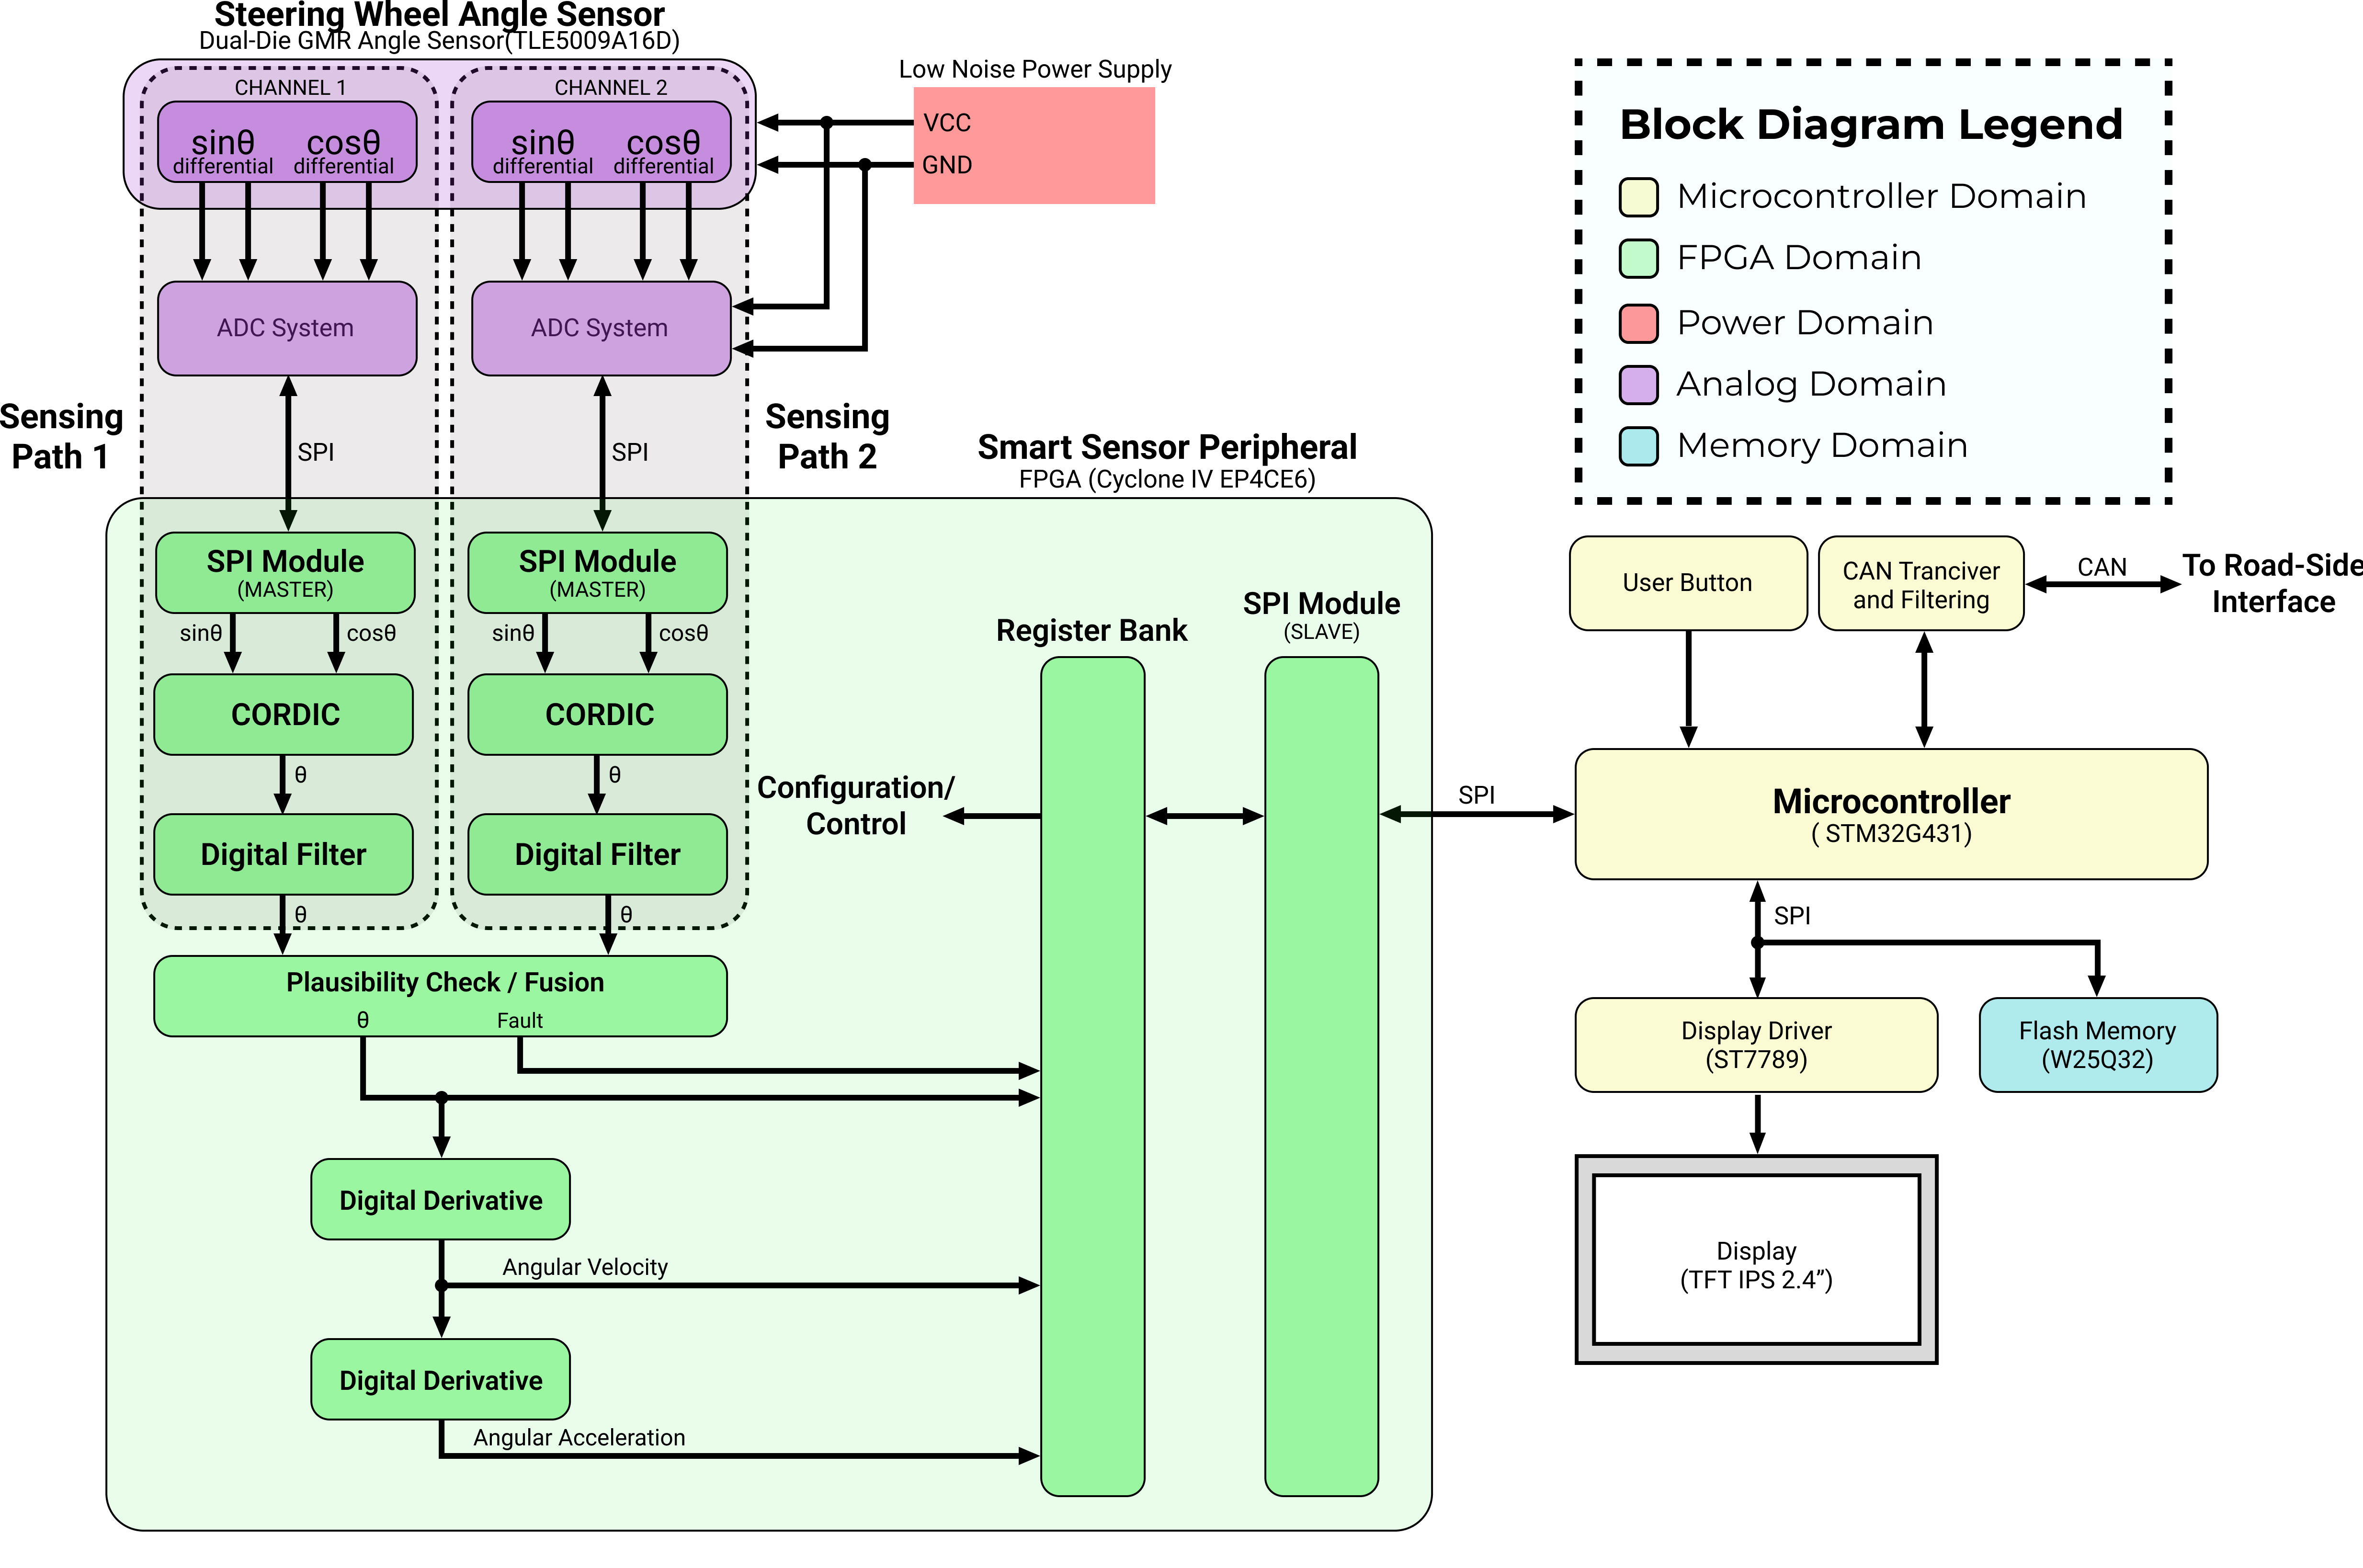
\includegraphics[width=1.0\linewidth]{figures/Human Side Block Diagram.jpg}
	\caption{Block diagram of the Human-Interaction Subsystem architecture.}
	\label{fig:human_side_block_diagram}
\end{figure}

The main architectural choices and the role of the different functional blocks are described in the following paragraphs.

\paragraph{FPGA-Based Smart Sensor Processing}
One of the main architectural choices of the Human-Interaction Subsystem is the use of an FPGA between the steering angle sensor and the main microcontroller. The FPGA is intended to implement the digital processing normally associated with a more advanced smart sensor.

Starting from the digitized sine and cosine signals generated by the steering sensor and the ADCs, the FPGA will process the measurements and provide higher-level information such as steering angle, angular velocity, angular acceleration and diagnostic status. These values will then be made available to the microcontroller through a register-based SPI interface. From the microcontroller point of view, the complete sensing subsystem can therefore be treated as a digital smart sensor, which directly provides already processed information through a standard communication interface.

In this way, the FPGA can be considered as a flexible implementation of the digital processing section of a smart sensing device. In a real-world application, similar functionality could also be implemented in an ASIC integrated with the sensor, while the use of an FPGA in this project makes it possible to directly design, test and modify the architecture.

\paragraph{Sensing Redundancy}
The Steering Wheel Angle Sensor is one of the main components of the Human-Interaction Subsystem, since its measurement is used to determine the steering request generated by the driver. For this reason, redundancy will be introduced in the sensing chain in order to improve fault detection and the overall dependability of the system.

The steering position will be measured using a dual-die angle sensor (TLE5009A16D), which integrates two separate sensing elements inside the same package. Each sensing channel generates analog sine and cosine signals, which are acquired through a dedicated ADC system and then processed inside the FPGA to obtain an estimation of the steering wheel angle. This complete sensing path is duplicated for the two channels of the sensor, generating two independent angle estimations.

The two resulting measurements are then compared through a plausibility check before generating the steering information made available to the microcontroller. A disagreement between the two channels can therefore be used to detect a possible fault in one of the sensing or acquisition paths.

It is important to note that the implemented redundancy is limited to the sensing and acquisition chain, and it is not applied at the system-level. Components such as the FPGA and the main microcontroller are still shared between the two channels, in practice impacting the dependability of the final architecture by introducing common failure modes. This choice was made because a fully redundant implementation would require the duplication of additional processing and control components, introducing a level of complexity that would not be justified within the scope of this project.


\paragraph{Human-Side Microcontroller}
The Human-Side Microcontroller (STM32G431) represents the main control unit of the subsystem and is responsible for the higher-level application logic of the whole Steer-by-Wire system. It combines data from the user inputs with feedback information received from the Road-Side Subsystem (such as the Vehicle Speed) in order to determine the target steering position to be requested from the Road-Side controller. The Road-Side Subsystem is then responsible for physically reaching this target according to the actual state and physical limitations of the actuator and steering mechanism.

In addition, the microcontroller manages the interaction with the driver through the display and buttons, handles configuration and diagnostic information, accesses the external non-volatile memory, and manages CAN communication with the Road-Side Subsystem.


\paragraph{Non-Volatile Memory}
An external non-volatile Flash memory (W25Q32) will be connected to the Human-Side Microcontroller in order to store information that must be preserved when the system is powered off. In particular, the memory will be used to store system configuration and calibration parameters, together with diagnostic and fault information generated during operation.

The memory also allows the system to maintain a persistent record of relevant events, which can later be accessed for diagnostic purposes. It will be directly managed by the microcontroller through an SPI interface.

It is important to note that, although the microcontroller already includes internal Flash memory, which could also be used to store persistent user data, an external Flash memory is intentionally used in this project to make the management of non-volatile data an explicit and independent part of the system architecture. This also allows the memory interface and management strategy to be designed independently from the specific microcontroller used.


\paragraph{CAN Communication}
The Human-Interaction Subsystem communicates with the Road-Side Subsystem, and potentially with other vehicle subsystems, through a CAN bus. The main information transmitted by the Human Side is the target steering position generated by the system-level control logic, while the Road-Side node sends feedback information related to the current steering state, actuator status, and vehicle status, such as vehicle speed.

CAN was selected because it is widely used in automotive embedded systems and is specifically suited for communication between distributed electronic control units. Its differential physical layer provides good immunity to electrical noise, while the protocol also includes mechanisms for error detection and reliable message transmission, which can be exploited to improve the overall dependability of the whole Steer-by-Wire system.

\paragraph{Power Supply}
In order to keep the block diagram as clear as possible, the power distribution architecture is not explicitly shown. The proposed system follows a typical automotive approach, described as follows: a common 12 V supply provided by a battery is distributed to the different electronic subsystems of the vehicle, with each node locally generating the voltage levels required by its components.

In particular, in the Human-Interaction Subsystem, a switching DC/DC converter will be used to efficiently step down the 12 V supply to the lower voltage rails required by the digital electronics. The exact voltage levels will depend on the final component selection.

In addition, since the steering sensing chain is particularly sensitive to electrical noise, a dedicated low-noise linear regulator (LDO) will also be used for the analog section containing the steering sensor and ADCs. This local supply is intended to reduce the switching noise reaching the acquisition circuitry and therefore improve the quality of the sensor measurements.












\section{Road-Side Subsystem}

As introduced in Section~\ref{overview}, the Road-Side Subsystem is responsible for the physical actuation of the steering system. Its main input is the target steering position generated by the Human-Interaction Subsystem and received through the CAN bus.

The subsystem locally controls the steering actuator in order to reach the requested position, using the steering position sensor as feedback. In addition, it acquires information related to the simulated vehicle state, such as the road speed, and sends relevant feedback and status information back to the Human-Interaction Subsystem via CAN.

The proposed architecture of the Road-Side Subsystem is shown in Figure~\ref{fig:road_side_block_diagram}.

\begin{figure}[H]
	\centering
	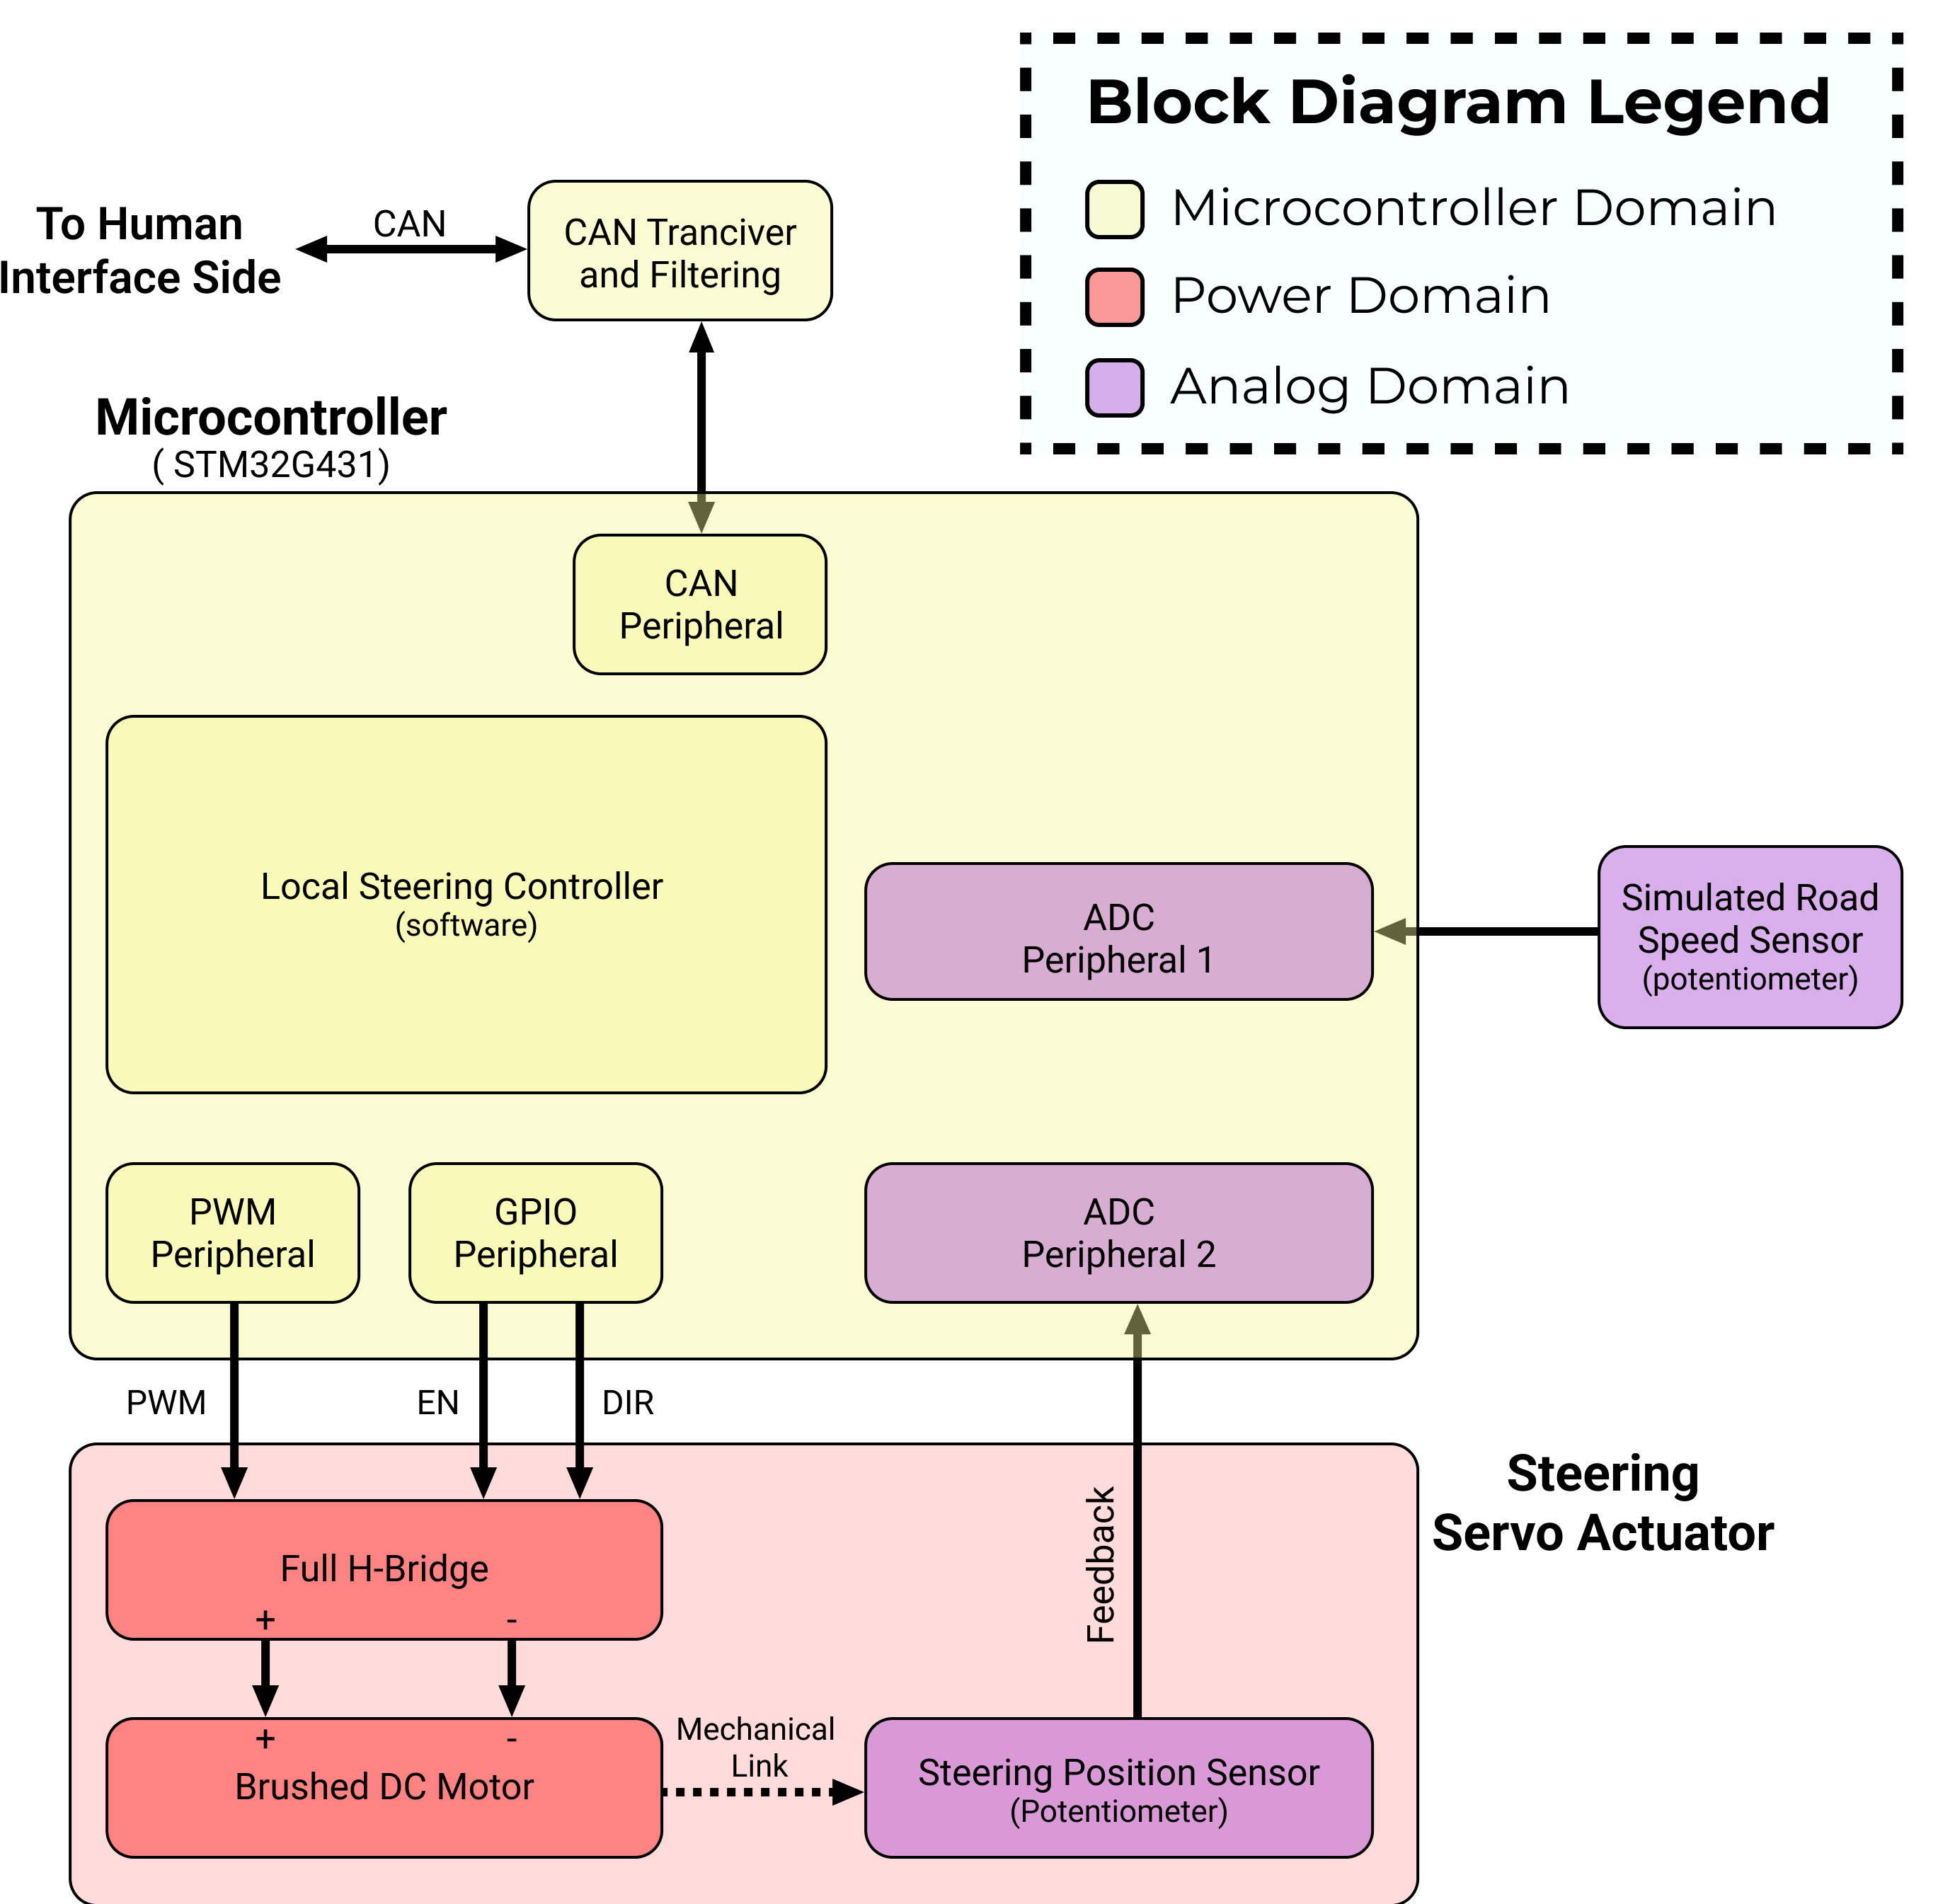
\includegraphics[width=0.7\linewidth]{figures/Road Side Block Diagram.jpg}
	\caption{Block diagram of the Road-Side Subsystem architecture.}
	\label{fig:road_side_block_diagram}
\end{figure}

The main architectural choices and the role of the different functional blocks are described in the following paragraphs.

\paragraph{Local Steering Controller}
The Road-Side Microcontroller implements the local steering control logic required to physically reach the steering position requested by the Human-Interaction Subsystem. The controller compares the target steering position received through the CAN bus with the actual steering position measured by the local feedback sensor, and uses this information to generate the commands for the steering actuator.

The objective of this local controller is to manage the physical behaviour of the actuator independently from the higher-level system logic. In particular, it is responsible not only for generating the PWM and direction commands used to drive the motor, but also for defining an appropriate motion strategy to reach the requested steering position in a controlled way. The controller must therefore take into account the actual steering position and the physical behaviour and limitations of the actuator and steering mechanism, for example by controlling how fast the target is approached and how the motion is slowed down when approaching the requested position.

\paragraph{Steering Servo Actuator}
The physical steering actuation is implemented as a closed-loop servo system composed of a brushed DC motor, a full H-bridge power stage, and a steering position sensor mechanically coupled to the steering mechanism.

The H-bridge allows the Road-Side Microcontroller to control the direction of rotation and the power delivered to the motor through the direction and PWM signals, therefore controlling the motion of the steering system. At the same time, the position sensor provides a direct measurement of the actual steering position reached by the mechanical system.

This measured position is used as feedback by the local controller and continuously compared with the requested target position. The motor command can therefore be adjusted during the movement in order to reach the requested steering position in a controlled and precise way.

\paragraph{Simulated Vehicle Speed}
In a real vehicle, information such as the vehicle speed would normally be provided by other electronic subsystems and exchanged through the vehicle communication network (usually implemented using CAN). In this demonstrator, this information will instead be simulated using a potentiometer connected to the Road-Side Microcontroller.

The simulated vehicle speed can then be transmitted to the Human-Interaction Subsystem and used by the system-level control logic to modify the steering behaviour according to the current vehicle state. This provides a simple way to test the interaction between the different subsystems without requiring the implementation of additional vehicle functions.





\section{Course Topics Coverage}

After describing the proposed architecture and the role of its main subsystems, it is useful to explicitly relate the implemented functionalities to the requirements of the final project. The following table summarizes this information:

\begin{table}[H]
	\centering
	\begin{tabular}{p{0.20\linewidth} p{0.75\linewidth}}
		\textbf{Course Topic} & \textbf{Project Implementation} \\ \hline
		Memories & External non-volatile Flash memory used for configuration, calibration and diagnostic data. \\
		
		Programmable Logic Devices & FPGA-based processing of the steering sensor signals, including angle estimation, filtering, plausibility checks and generation of higher-level sensor information. Design of a peripheral-like interface, accessible via SPI\\
		
		Interconnections & SPI communication between different devices (Display, Flash Memory, FPGA sensor peripheral) and CAN communication between the Human-Interaction and Road-Side subsystems. \\
		
		Processor Peripherals & Use of microcontroller peripherals such as ADC, CAN and timer/PWM modules for sensing, communication and actuator control. 2 separate microcontrollers are used, one for each main subsystem\\
		
		A/D Conversion & External ADC systems used to acquire the analog sine and cosine signals generated by the steering angle sensor. \\
		
		Power Management & Switching power conversion for the electronic subsystems and full H-bridge driving of the steering actuator. \\
	\end{tabular}
\end{table}